% !TeX spellcheck = en_US

% Document settings
\documentclass[sigconf]{acmart}

% Microtype settings
\usepackage{microtype}

% Language settings
\usepackage[american]{babel}
\usepackage[utf8x]{inputenc}
\usepackage[T1]{fontenc}

% Quotes settings
\usepackage{csquotes}

% Comments settings
\usepackage{verbatim}

% Numbers settings
\usepackage[binary-units]{siunitx}
\usepackage[super]{nth}

% Math settings
\usepackage{amsmath}
\usepackage{amssymb}

% Images settings
\usepackage{float}
\usepackage{graphicx}

% Tables settings
\usepackage{booktabs}
\usepackage{multirow}

% Bibliography settings
\bibliographystyle{ACM-Reference-Format}

% Lists settings
\usepackage{paralist}
\usepackage{enumitem}
\usepackage{xcolor}
% Circles characters settings
\usepackage{tikz}
\newcommand*\circled[1]{\tikz[baseline=(char.base)]{\node[shape=circle,draw,inner sep=1pt] (char) {#1};}}

% Balancing settings
%\usepackage[keeplastbox]{flushend}

% Custom commands
\usepackage{xparse}
\usepackage{xspace}
\NewDocumentCommand{\eg}{}{e.g.\@\xspace}
\NewDocumentCommand{\ie}{}{i.e.\@\xspace}
\NewDocumentCommand{\etal}{}{et al.\@\xspace}
\NewDocumentCommand{\req}{m}{\textbf{RQ#1}\@\xspace}
\NewDocumentCommand{\TODO}{m}{\textcolor{red}{TODO:#1}\@\xspace}

% Links and PDF settings
\usepackage{hyperref}
\hypersetup{
	hidelinks,
	pdftitle={Temporary Title},
	pdfauthor={Temporary Author 1, Temporary Author 1},
	pdfkeywords={Keyword1, Keyword2}
}
\usepackage[all]{hypcap}

% URL formatting
\usepackage{url}

\begin{document}
	% !TeX spellcheck = en_US

\acmConference[GECCO '17]{the Genetic and Evolutionary Computation Conference 2017}{July 15--19, 2017}{Berlin, Germany}
\acmYear{2017}
\copyrightyear{2017}

	
	% !TeX spellcheck = en_US

\title{Exploiting Subprograms in Genetic Programming}

	% !TeX spellcheck = en_US

\author{Steven Fine}
\orcid{1234-5678-9012}
\affiliation{%
	\institution{Massachusetts Institution of Technology, USA}
}
\email{sfine@mit.edu}

\author{Erik Hemberg}
\orcid{1234-5678-9012}
\affiliation{%
	\institution{Massachusetts Institute of Technology, USA}
}
\email{hembergerik@csail.mit.edu}

\author{Una-May O'Reilly}
\orcid{1234-5678-9012}
\affiliation{%
	\institution{Massachusetts Institute of Technology, USA}
}
\email{unamay@csail.mit.edu}

	% !TeX spellcheck = en_US

\begin{abstract}
ABSTRACT GOES HERE.
\vspace{1.5in}


\end{abstract}

	 !TeX spellcheck = en_US

	% !TeX spellcheck = en_US

\keywords{Keyword 1, Keyword 2}

	\maketitle
	
	\newcommand{\st}{subprogram\xspace} 

\section{Introduction}\label{sect:intro}
%Genetic programming is a general algorithmic technique in which the principles of neo-Darwinian evolution are translated  to algorithmic form in order to generate programs of specific functionality. 
Our general goal is to improve the level of program complexity that genetic programming(GP) can routinely evolve\cite{koza1992genetic}. This is toward fulfilling its potential to occupy a significant niche in the ever advancing field of program synthesis\cite{weimer2010automatic, rinard2012example, gulwani2010dimensions}.  Behavioral genetic programming (BGP) is an extension to GP that advances toward this compelling goal\cite{krawiecGecco2014,KrawiecBPS2016}. The intuition of the BGP paradigm is that, during evolutionary search and optimization, information characterizing programs by behavioral properties that extend beyond how accurately they match their target outputs. This information from a program ``trace'' can be effectively integrated into extensions of the algorithm's fundamental mechanisms of fitness-based selection and genetic variation. 

To identify useful subprograms BGP commonly exploits program \textit{trace} information (first introduced in \cite{krawiec2013pattern} which is a capture of the output of every subprogram within the program for every test data point during fitness evaluation.  %Consider a simple program, which computes the mathematical function $f(x) = \ln(x1) + (x1 - x2)$ and the sample data set in Table \ref{table:sample_data}. Conventional genetic programming will only consider the outputs for each data point: $\ln(3) + 1$, $\ln(5) + 2$, and compare those values to the desired output.  However, each subtree has its own output, which is ignored by the genetic programming process. 
%\begin{table*}[ht]
%\centering
%\begin{tabular}{ c c | c }
%\hline\hline
%$x_{1}$ & $x_{2}$ & $y$ \\ [0.5ex]
%\hline
%3 & 2 & 3 \\
%5 & 3 & 4 \\[1ex]
%\hline
%\end{tabular}
%\caption{Sample data set.}
%\label{table:sample_data}
%\end{table*}
%
%The collection of the outputs on each subtree for all of the data points is called the trace.  For the program in Figure \ref{figure:gp_tree} and the fitness cases in Table \ref{table:sample_data}, the trace is shown in Table \ref{table:sample_trace}.
%
%\begin{table*}[ht]
%\centering
%\begin{tabular}{ c c c c c c }
%\hline\hline
%$s_{1}$ & $s_{2}$ & $s_{3}$ & $s_{4}$ & $s_{5}$ & $s_{6}$ \\ [0.5ex]
%\hline
%3 & $\ln(3)$ & 3 & 2 & 1 & $\ln(3)$ + 1 \\
%5 & $\ln(5)$ & 5 & 3 & 2 & $\ln(5)$ + 2 \\[1ex]
%\hline
%\end{tabular}
%\caption{The trace of the program from Figure \ref{figure:gp_tree} for the data set in Table \ref{table:sample_data}.}
%\label{table:sample_trace}
%\end{table*}
The trace is stored in a matrix where the number of rows is equal to the number of test suite data points, and the number of columns is equal to the number of subtrees in a given program. % There is no set order of the columns, although here they are presented in the depth first traversal order of the subtrees that produce the values.  
The trace captures a full snapshot of all of the intermediate states of the program evaluation. 

BGP then uses the trace to estimate the merit of each subprogram by treating its column as a feature (or explanatory variable) in a \textit{model regression} on the desired program outputs.  The accuracy and complexity of the model reveals how useful the subprograms are. The model, if it has feature selection capability, also reveals  specific subprograms within the tree that are partially contributing to the program's fitness.  BGP uses this information in two ways. It can integrate \textit{model error }and \textit{model complexity} into the program's fitness. Second, it maintains an archive of the most useful subtrees identified by modeling each program and uses them in an \textit{archive-based crossover}. BGP has a number of variants that collectively yield impressive results, see \cite{krawiecGecco2014,KrawiecBPS2016}. 

%It demonstrates that we should look at how a program behaves during execution because partial behavior, if it can be identified and isolated, can be used to direct GP toward better program synthesis. 
%  move previous sentence to conclusion? redundant here?
\newcommand{\ct}{$T^c$}
%BGP is a paradigm rich with possible extensions to explore, many of which could give deeper insight into genetic programming synthesis methods. 

In this work,  we explore various extensions to the BGP paradigm that are motivated by 2 central topics: \begin{inparaenum}

\item \textbf{The impact of bias from the inference model on useful subprogram identification and program fitness.}  Model techniques and even the implementation of the same technique can differ in  \textit{bias}, i.e. error from assumptions in the learning algorithm, e.g. implementation of a ``decision tree'' algorithm. These differences, in turn, impact which subprograms are inserted/retrieved from the BGP archive and the model accuracy and model complexity factors that are integrated into a program's fitness. Therefore, we investigate how much BGP is sensitive to model bias. %in terms of its impact on estimations of merit for subprograms and the ensuing integration of this estimates in program fitness and archiving and crossover.  
\textit{How important is it which subprograms the model technique selects and how accurate a model is? }  We answer these questions by comparing BGP competence under 2 different implementations of decision tree modeling which we observe have different baises. Our investigation contrasts feature identification and model accuracy under the two implementations. 

\item \textbf{``Plays well with others?''}: \textbf{Alternate ways to identify useful subprograms}. BGP uses the trace matrix from a program implying all the subprograms of one program are treated as a set of features during modeling. This means that feature selection and subprogram fitness estimation occurs within the program context.  Essentially, each subprogram is juxtaposed with ``relatives'' -- its parent, neighbors and even child in GP tree terms. Does this context provide the best means of identifying useful subprograms? It may not. Crossover moves a subprogram into another program so, to work most effectively, it should explore recombinations of subprograms that \textit{work well in other subprograms and programs in the population}. We examine this idea by concatenating program traces from a set of programs, not solely one program. This demands a new measure of fitness to reflect subprogram participation in the model as a means of archive selection and program fitness. We examine concatenation of the entire population and sub-populations based on fitness to ask whether fitter programs with concatenated traces are more effective than an open playing field. i.e. the entire population of subprograms.  
  %Perhaps program context does not reflect how well a subprogram ``\textit{plays with other subprograms in the population}''.
\end{inparaenum}

Our specific demonstration focus herein is  symbolic regression. We choose SR because it remains a challenge and have good benchmarks~\cite{benchmarks} so it allows us to measure progress and extensions. It also has real world application to system identification and, with modest modification, machine learning regression and classification.  In passing, we replicate BGP logic, making our project software available with an open source license.

We proceed as follows: \TODO{INSERT ROADMAP} 
\vspace{1.0in}


	\section{Related Work (one column)}
\label{sec:related-work}

BGP is not the only approach to program synthesis, there are e.g. sketching\cite{solar2008program}, i.e. communicating insight through a partial program, generalized program verification\cite{srivastava2010program}, as well as hybrid computing with neural network and external menory\cite{graves2016hybrid}

One extension to the genetic programming paradigm is behavioral
genetic programming (BGP) \cite{krawiecGecco2014,KrawiecBPS2016}.  BGP
attempts to identify useful subprograms that can then be used to
enhance the evolutionary process. The behaviroal program syhnthesis
with Genetic Programming\cite{krawiec2016behavioral} is investigated,
where the goal is to automatically generate a program that meets some
requirements. E.g. BGP looks at implicit fitness
sharing\cite{mckay2000fitness}, trace consistency analysis, memory in
the form of archives\cite{haynes1997line}. Extension of BGP are
e.g. Memetic Semantic Genetic
Programming\cite{Ffrancon:2015:MSG:2739480.2754697}.

Since its inception\cite{krawiec2013pattern} and the introduction of
the trace matrix and demonstration in a system called PANGEA where
minimum description length was induced from the program execution,
there have been a variety of extensions. For example, in the general
vein of behaviorally characterizing a program by more than its
accuracy, e.g. when discovering search objectives for test-based
problems\cite{liskowski2016online}.

The relationship between BGP and Semantic GP is the common goal of
characterising program behaviour in more detail, and exploit this
information. Wheras BGP looks at subprograms semantic GP, where
program output is scrutinized for every test individually, was
initiated by a study of the impact of crossover on program semantics
and semantic building blocks~\cite{mcphee2008semantic}. A survey of
semantic models in GP~\cite{vanneschi2014survey} gives an overview of
methods for operators, as well as different objectives.


	\section{Exploiting Subprograms}\label{sect:foreground}
\subsection{BGP Strategy}
What emerges from the details of BGP's successful examples is a stepwise strategy:  
\begin{inparaenum}

\item For each program in the population, capture the behavior of each \st{s} in a trace matrix $T$.

\item  Regress $T$ as feature data on the desired program outputs and derive a model $M$. 

\item Assign a value of merit $w$ to each \st in $M$. Use this merit to determine whether it should be inserted into an archive. Use a modified crossover that draws subprograms from the archive. 

\item Integrate model error $e$ and complexity $c$ into program fitness.
\end{inparaenum} \\

% WEKA Citation M. Hall, E. Frank, G. Holmes, B. Pfahringer,
%P. Reutemann, and I. H. Witten. The weka data mining software: An update. SIGKDD Explor. Newsl., 11(1):10–18, Nov. 2009.

One example of the strategy is realized in \cite{krawiecGecco2014} where, in Step~(2), the fast RepTree (\REPTREE - Reduced  Error  Pruning  Tree) algorithm  of decision tree classification from the WEKA Data Mining software library\cite{Hall:2009:WDM:1656274.1656278} is used for regression modeling.  \REPTREE builds a decision/regression tree using information gain/variance. In Step~(3) merit is measured per Equation~\ref{eq:subtree_weight} where $|U(p)|$ is the number of subprograms (equivalently distinct columns of the trace) used in the model and $e$ is model error.


\begin{equation}
\label{eq:subtree_weight}
w = \frac{1}{(1 + e)|U(p)|}
\end{equation}

\subsection{Exploring Model Bias}
Following our motivation to understand the impact of model bias on useful subprogram identification and program fitness, we first explore an alternative realization of BGP's strategy by using the \SCIKIT optimized version of the CART decision tree algorithm\footnote{\url{http://scikit-learn.org/stable/modules/tree.html\#tree-algorithms-id3-c4-5-c5-0-and-cart}}.  CART (Classification and Regression Trees) is very similar to C4.5, but it differs in that it supports numerical target variables (regression) and does not compute rule sets. CART constructs binary trees using the feature and threshold that yield the largest information gain at each node.  With the \SCIKIT implementation we derive a model in the same manner that we derive a model from \REPTREE.  We denote the model derived for \SCIKIT by $M_S$ and contrast it with the model derived from \REPTREE, which we now denote by $M_R$.

\subsection{Identifying Useful Subprograms}
\newcommand{\FULL}{\textbf{FULL}\xspace}
\newcommand{\DRAW}{\textbf{DRAW}\xspace}
Next we realize alternative implementations of the BGP strategy. We do this to investigate alternative ways of identifying useful subprograms, considering that prior work only considers models that are trained on the trace of a single program. In Step~(1) we first select a set of programs  $C$ from the population. We then form a new kind of trace matrix, $T_c$, by column-wise concatenating all $T${'s} of the programs in $C$. In a version we call \FULL,  $T_c$ is then passed through Step~(2). We proceed with step (3), but it is important to note that the weights given to the subprograms considered for the archive are identical, because only a single model is built. Step (4) is altered to incorporate model contribution in place of model error and complexity. The model is built from the features of many programs, so the model error and model complexity for each individual program are undefined. Model contribution measures how many features each program contributes to $M$.  For this we use $w_{c}$, which is given by Equation~\ref{eq:subtree_contrib}, where $p'$ is the number of features in $M$ from program $p$, and $|U(M)|$ is the total number of features from $T_{c}$ used in $M$. This method allows us to experiment with different programs in $C$, trying $C$ containing all the programs in the population, for diversity and, conversely trying elitism, holding only a top fraction of the  population by fitness. 

% $x\%$ by fitness (as computed by NSGA2 pareto crowding ordering) where $x$ ranges from 25\% of the population to a less elite shares of $50\%$ and $75\%$.

\begin{equation}
\label{eq:subtree_contrib}
w_c = 1 - \frac{p'}{|U(M)|}
\end{equation}

An alternative implementation, that we name \DRAW,  is to draw random subsets from $T_{c}$, and build a model on each.  This would possibly contribute to a more robust archive, if it can be populated with subtrees that are frequently selected by the machine learning model.  We modify Step~(3) to account for the possibility that a specific subtree was chosen to be in more than one model.  In this case, the subtree's merit $w$ is set to be the sum of the assigned merit values each time the subtree is chosen.  Step~(4) is modified in the same way as it is in \FULL.

Implementation details of \FULL and of \DRAW are provided the next section.  


%Initially $U$ will be the entire population.

	
\section{Experiments}\label{sect:experiments}

We start this section by detailing the benchmarks we use, the parameters of our algorithms and name our algorithm configurations for convenience. Section~\ref{sect:ftr-select} then evaluates the impact of different decision tree algorithms. Section~\ref{sect:agg-features} evaluates the performance of \FULL and \DRAW for different configurations then compares \FULL, \DRAW and program-based model techniques.
 
\subsection{Experimental Data, Parameters}\label{sect:data_sets}

Our investigation uses 17 symbolic regression benchmarks from~\cite{benchmarks}. All of the benchmarks are defined such that the dependent variable is the output of a particular mathematical function for a given set of inputs.  All of the inputs are taken to form a grid on some interval.  Let $E[a, b, c]$ denote $c$ samples equally spaced in the interval $[a,b]$. (Note that McDermott et al. defines $E[a, b, c]$ slightly differently.)  Below is a list of all of the benchmarks that are used:

\begin{enumerate}
\item \textbf{Keijzer1}: $0.3x \sin(2 \pi x);$ $x \in E[-1,1,20]$
\item \textbf{Keijzer11}: $x y+\sin((x-1)(y-1));$ $x, y \in E[-3,3,5]$
\item \textbf{Keijzer12}: $x^{4}-x^{3}+\frac{y^{2}}{2}-y;$ $x, y \in E[-3,3,5]$
\item \textbf{Keijzer13}: $6 \sin(x) \cos(y);$ $x, y \in E[-3,3,5]$
\item \textbf{Keijzer14}: $\frac{8}{2 + x^{2} + y^{2}};$ $x,y \in E[-3,3,5]$
\item \textbf{Keijzer15}: $\frac{x^{3}}{5} - \frac{y^{3}}{2} - y - x;$ $x, y \in E[-3,3,5]$
\item \textbf{Keijzer4}: $x^{3} e^{-x} \cos(x) \sin(x) (\sin^{2}(x) \cos(x) - 1);$ $x \in E[0,10,20]$
\item \textbf{Keijzer5}: $\frac{3 x z}{(x - 10) y^{2}};$ $x,y \in E[-1,1,4]; z \in E[1,2,4]$
\item \textbf{Nguyen10}: $2 \sin(x) \cos(y);$ $x,y \in E[0,1,5]$
\item \textbf{Nguyen12}: $x^{4} - x^{3} + \frac{y^{2}}{2} - y;$ $x,y \in E[0,1,5]$
\item \textbf{Nguyen3}: $x^{5} + x^{4} + x^{3} + x^{2} + x;$ $x \in E[-1,1,20]$
\item \textbf{Nguyen4}: $x^{6} + x^{5} + x^{4} + x^{3} + x^{2} + x;$ $x \in E[-1,1,20]$
\item \textbf{Nguyen5}: $\sin(x^{2}) \cos(x) - 1;$ $x \in E[-1,1,20]$
\item \textbf{Nguyen6}: $\sin(x) + \sin(x + x^{2});$ $x \in E[-1,1,20]$
\item \textbf{Nguyen7}: $\ln(x + 1) + \ln(x^{2} + 1);$ $x \in E[0,2,20]$
\item \textbf{Nguyen9}: $\sin(x) + \sin(y^{2});$ $x,y \in E[0,1,5]$
\item \textbf{Sext}: $x^{6} - 2 x^{4} + x^{2};$ $x \in E[-1,1,20]$
\end{enumerate}

We use a standard implementation of GP and chose parameters according to settings documented in~\cite{krawiecGecco2014}.


\textbf{Fixed Parameters}\label{appendix:fixed_parameters}
\begin{itemize}
\item \textbf{Tournament size}: 4
\item \textbf{Population size}: 100
\item \textbf{Number of Generations}: 250
\item \textbf{Maximum Program Tree Depth}: 17
\item \textbf{Function set}\footnote{Note that for our implementation of $/$, if the denominator is less than $10^{-6}$ we return $1$, and for our implementation of $\log$, if the denominator is less than $10^{-6}$ we return $0$.}: $\{ +, -, *, /, \log, \exp, \sin, \cos, -x \}$
\item \textbf{Terminal set}: Only the features in the benchmark.
\item \textbf{Archive Capacity}: 50
\item \textbf{Mutation Rate $\mu$}: 0.1
\item \textbf{Crossover Rate with Archive configuration $\chi$}: 0.0
\item \textbf{Crossover Rate with GP $\chi$}: 0.9
\item \textbf{Archive-Based Crossover Rate $\alpha$}: 0.9
\item \textbf{REPTree}  defaults but no pruning
\item \textbf{\SCIKIT} defaults
\item \textbf{Number of runs} 30
\end{itemize}

First we use the 3 BGP algorithm configurations that use \REPTREE to replicate \cite{krawiecGecco2014}'s work on the symbolic regression benchmarks. These we call BGP2A, BGP4, BGP4A following precedent. In the name the digit 2 indicates that model error $e$ and complexity $c$ were not integrated into program fitness while 4 indicates they were.   The suffix A indicates whether or not subprograms from the model were qualified for archive insertion and archive retrieval during BGP crossover. When the A is omitted ordinary crossover is used. We observe results consistent with the prior work. Our open source software is available on Github.
This allowed us to proceed to evaluate feature selection sensitivity based on modeling algorithm.

It is important to note, that for each configuration we report regression, i.e. training set performance. We are primarily interested in exploring subprogram behavior and how to assemble subprograms. Reporting generalization would complicate the discussion without materially affecting our conclusions. 

\subsection{Sensitivity to Model Bias}\label{sect:ftr-select}

Q1. Does the feature selection bias of the model step matter? 

\begin{table}[ht]
\centering
\small
\begin{tabular}{ c | c c c }
\hline\hline
& Configuration & & Average Rank \\
\hline
1 & BP2A & \REPTree & 1.82 \\
2 & BP2A & \SCIKIT  & 2.94 \\
3 & BP4A & \SCIKIT  & 3.06 \\
4 & BP4 & \SCIKIT  & 3.18 \\
5 & BP4A & \REPTree & 4.65 \\
6 & BP4 & \REPTree & 5.35 \\
\end{tabular}
\caption{Comparison of impact of \REPTree vs \SCIKIT for average fitness rank across all data sets.}
\label{table:ranksReTreeVCART}
\end{table}


Table~\ref{table:ranksReTreeVCART} shows the results of running the 3 different configurations (BGP2A, BGP4, BGP4A) each with the two decision tree algorithms.  Averaging over the rankings across each benchmark we find that BP2A using \REPTREE is best. For BPG2A, \REPTREE outranks \SCIKIT but when model error is integrated into the program fitness, (i.e. BPG4A and BPG4) regardless of whether or not an archive is used, \SCIKIT is superior to \REPTREE.  

When we compare the results of using the archive while model error is integrated into the program fitness (i.e.  BPG4A to BPG4), for both \REPTREE and \SCIKIT it is better to use an archive than to forgo one.  Comparing BPG2A with BPG4A, we can measure the impact of model error and complexity integration.  We find that for both \SCIKIT and \REPTREE it is not helpful to integrate model error and complexity into program fitness. 

For a deeper dive, at the specific benchmark level, Table~\ref{table:fitnessReTreeVCART} shows the average best fitness at end of run (of 30 runs), for each benchmark.   Averaging all fitness results, no clear winner is  discernible. For certain comparisons \SCIKIT will be superior while for others \REPTREE is.   We also show one randomly selected run of Keijzer1 running with \REPTREE modeling and configuration BPG4 in Figure~\ref{fig:deepdive}.   We plot on the first row  model error on the left and the fitness of the best program (right).  The plots on the second row show number of features of model  and number of subprograms in the best program (right). The plots on the third row show the ratio of number of model features to program subtrees (left) and ratio of model error to program fitness. Since the run is configured for  BPG4 program fitness integrates both model error and complexity.  No discernible difference arose among this sort of plot. This is understandable given the stochastic nature of BGP.

\begin{table*}[ht]
\centering
%\begin{adjustbox}{width=1\textwidth}
\tiny
%\begin{tabularx}{\linewidth}{|>{\RaggedRight}p{2.5cm}|x|x|x|}\hline
\begin{tabular}{ c c c c c c c c c c c c c c c c c c c }
\hline\hline
 & & Keij1 & Keij11 & Keij12 & Keij13 & Keij14 & Keij15 & Keij4 & Keij5 & Nguy10 & Nguy12 & Nguy3 & Nguy4 & Nguy5 & Nguy6 & Nguy7 & Nguy9 & Sext \\
\hline
BP2A & \REPTree & \textbf{0.243} & 0.776 & 0.972 & \textbf{0.393} & 0.723 & \textbf{0.883} & \textbf{0.384} & \textbf{0.975} & \textbf{0.11} & \textbf{0.343} & 0.196 & \textbf{0.265} & 0.037 & 0.091 & 0.122 & 0.068 & \textbf{0.052} \\
 & \SCIKIT & 0.327 & 0.769 & \textbf{0.966} & 0.481 & 0.726 & 0.907 & 0.468 & 0.977 & 0.199 & 0.379 & 0.2 & 0.285 & 0.04 & 0.119 & 0.127 & 0.075 & 0.054 \\
BP4 & \REPTree & 0.359 & 0.852 & 0.982 & 0.817 & 0.872 & 0.922 & 0.522 & 0.993 & 0.309 & 0.388 & \textbf{0.193} & 0.33 & 0.103 & 0.133 & 0.117 & 0.165 & 0.127 \\
 & \SCIKIT & 0.357 & \textbf{0.684} & 0.968 & 0.548 & 0.776 & 0.887 & 0.513 & 0.991 & 0.144 & 0.36 & 0.266 & 0.288 & 0.126 & \textbf{0.0} & \textbf{0.104} & \textbf{0.04} & 0.083 \\
BP4A & \REPTree & 0.319 & 0.804 & 0.981 & 0.765 & 0.821 & 0.919 & 0.505 & 0.991 & 0.209 & 0.386 & 0.22 & 0.328 & 0.088 & 0.117 & 0.128 & 0.194 & 0.1 \\
 & \SCIKIT & 0.261 & 0.811 & 0.973 & 0.507 & \textbf{0.691} & 0.94 & 0.471 & 0.981 & 0.264 & 0.379 & 0.219 & 0.273 & \textbf{0.034} & 0.088 & 0.115 & 0.065 & 0.056 \\
\hline
\end{tabular}
%\end{adjustbox}
\caption{Comparison of different decision tree algorithms: \REPTREE and \SCIKIT on average program error for best of run programs (averaged across 30 runs). N.B. program error does NOT include program size. During evolution the fitness of a program integrates program error and size per\cite{krawiecGecco2014}}
\label{table:fitnessReTreeVCART}
\end{table*}


\begin{figure}[htbp]
\begin{center}
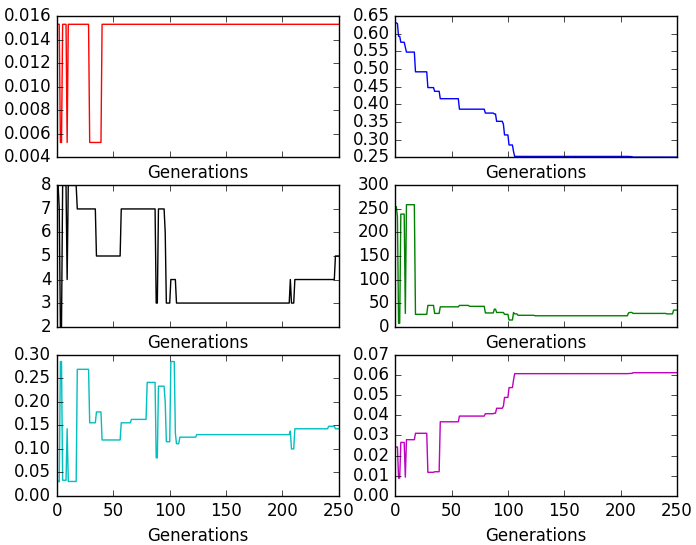
\includegraphics[width=0.99\linewidth]{sections/figures/figure_reptree.png}
\caption{We take one run of Keijzer1 running with \REPTREE modeling and configuration BP4.   We plot on the first row  model error on the left and the fitness of the best program (right).  The plots on the second row show number of features of model  and number of subprograms in the best program (right). The plots on the third row show the ratio of number of model features to program subtrees (left) and ratio of model error to program fitness. Since the run is configured for  BP4 program fitness integrates both model error and complexity.}
\label{fig:deepdive}
\end{center}
\end{figure}

%
%Describe difference in implementations between Reptree and SKL-RepTree.\\
%Need REPTREE and Scikit learn algorithm references and links to their code.
%
%Compare REPTREE TO SICKIT LEARN for BGP 2A, 4a, 4 getting 6 combinations\\
%Reference Table~\ref{table:avg_fitness} comparing average program error among BGP2A, BGP4, BGP4A, GP for 17 functions with REPTREE and ScikitLearn implementation.\\
%Reference Table~\ref{table:avg_size} showing average program size among BGP2A, BGP4, BGP4A, GP for 17 functions with REPTREE and ScikitLearn implementation.\\
%STDEV is in separate table in thesis, how to handle in paper?
%
%Statistical testing required!!
%
%Include a ranking table.  just on error of program and only 6 combinations (two choices of decision tree implementation) and 3 algorithms (2A,4,4A). 
%
%Select 1 run, 1 dataset: what is \# of features in model of best individual at first and final generation (each generation)? What is fraction of \# of features in model to \# of subtrees in best individual at first and final generation (each generation)?  (Each generation) means we would have a plot (fitness on Y1 axis, features/fraction on Y2, Y3 and X is generations). We could amass these statistics for every dataset and 30 runs but lower priority than other tasks.
%
We conclude that in this case of different decision tree algorithms perhaps the subtlety of contrast is not strong enough.  

\subsection{Aggregate Trace Matrices}\label{sect:agg-features}
In this section, we compare various configurations of \FULL and \DRAW.  For the algorithm configurations of this section, we adopt a clearer notation. We drop the BGP prefix and use $M$ to denote when program contribution is integrated into program fitness, and $\hat M$ to denote when it is not. We use $A$ to denote when subprograms are qualified for archive insertion and archive retrieval during BGP crossover, and $\hat A$ to denote when ordinary crossover is used.

More details of the \DRAW method are appropriate.  Referencing \cite{krawiecGecco2014} we analyze the formula for computing the weight of a given subtree (see Equation~\ref{eq:subtree_weight}).  We note that the $|U(p)|$ factor in its denominator indirectly increases the weight of smaller subprograms.  This occurs because smaller programs yield smaller models (i.e. smaller $|U(p)|$), and smaller programs have smaller subprograms.  Therefore we designed \DRAW to also favor the archiving of smaller subprograms.  \DRAW proceeds as follows:

\begin{inparaenum}
\item The population is sorted best to worst by program fitness (program error and size) using the NSGA pareto front crowding calculation because BGP is multi-objective.

\item The sorted population is cut off from below at a threshold $\lambda \%$ to form $C$.  The trace matrixes of every program in $C$ are concatenated to form $T_C$ which we call the subprogram pool.  

\item We next sort the population by \textbf{size} and select the smallest $20\%$ forming a size sample we call $K$.
   
\item Finally we draw from $K$ at random to obtain the number of subprograms that will be collectively modeled. Then we select the equivalent number of columns at random from $T_C$ and form a model. We repeat this step each time for the size of the population.  This generates multiple smaller collections of diverse subprograms. 

\end{inparaenum}

\noindent Q2. Can trace matrix concatenation which pools subprograms among different programs improve BGP performance?


\begin{table*}[ht]
\centering
%\begin{adjustbox}{width=1\textwidth}
\small
\begin{tabular}{ c | c c c ||  c c c c }
 $C$& $\hat M A$ & $M \hat A$ & $MA$ & $\hat M A$ & $M \hat A$ & $MA$\\ \hline
 25 & 3.06 & 2.24 & 2.35 & \textbf{1.65} & 2.18 & \textbf{1.41} \\
 50 & \textbf{2.29} & \textbf{1.82} & \textbf{1.88} & 2.41 & \textbf{1.88} & 2.29 \\
 75 & \textbf{2.29} & 2.0 & 2.0 & 3.06 & 2.12 & 2.65 \\
 100 & 2.35 & 3.94 & 3.76 &2.88 & 3.82 & 3.65  \\
%\hline
\end{tabular}
%\end{adjustbox}
\caption{\DRAW (lhs) and \FULL (rhs) average rank varying model fitness signal (M or $\hat M$) and use of archive (A or $\hat A$) for 17 benchmarks}
\label{table:XXdraws_avg_ranks}
\end{table*}


%\input{sections/fullpop_average_ranks}

\begin{table*}[ht]
\tiny
\centering
%\begin{adjustbox}{width=1\textwidth}
\begin{tabular}{ c | c | c c c c c c c c c c c c c c c c c }
%\hline\hline
 & & Keij1 & Keij11 & Keij12 & Keij13 & Keij14 & Keij15 & Keij4 & Keij5 & Nguy10 & Nguy12 & Nguy3 & Nguy4 & Nguy5 & Nguy6 & Nguy7 & Nguy9 & Sext \\
 \hline
& Draw 25 & 0.306 & 0.704 & 0.976 & 0.436 & 0.768 & \textbf{0.845} & 0.371 & 0.975 & 0.162 & 0.341 & \textbf{0.172} & 0.301 & 0.056 & 0.074 & 0.132 & 0.241 & 0.058 \\
$\bar M A$ & Draw 50 & 0.286 & \textbf{0.604} & 0.969 & 0.422 & 0.731 & 0.866 & 0.376 & \textbf{0.967} & 0.107 & 0.353 & 0.194 & 0.295 & 0.045 & 0.089 & \textbf{0.103} & 0.159 & 0.059 \\
 & Draw 75 & \textbf{0.246} & 0.716 & 0.968 & \textbf{0.325} & 0.736 & 0.869 & 0.347 & 0.974 & \textbf{0.089} & 0.351 & 0.215 & 0.278 & 0.06 & 0.1 & 0.118 & 0.206 & \textbf{0.044} \\
 & Draw 100 & 0.253 & 0.695 & 0.969 & 0.382 & \textbf{0.716} & 0.877 & \textbf{0.33} & 0.972 & 0.123 & 0.356 & 0.217 & 0.285 & \textbf{0.03} & 0.129 & 0.115 & 0.165 & 0.047 \\
 \hline
 & Full 25 & 0.278 & 0.812 & \textbf{0.956} & 0.621 & 0.761 & 0.88 & 0.457 & 0.977 & 0.232 & 0.385 & 0.297 & 0.33 & 0.058 & 0.159 & 0.204 & 0.212 & 0.062 \\
 & Full 50 & 0.279 & 0.883 & 0.979 & 0.564 & 0.748 & 0.921 & 0.411 & 0.981 & 0.294 & 0.387 & 0.337 & 0.37 & 0.06 & 0.264 & 0.195 & 0.301 & 0.086 \\
 & Full 75 & 0.302 & 0.864 & 0.976 & 0.604 & 0.804 & 0.925 & 0.453 & 0.982 & 0.364 & 0.395 & 0.316 & 0.361 & 0.059 & 0.271 & 0.225 & 0.306 & 0.088 \\
 & Full 100 & 0.272 & 0.864 & 0.982 & 0.565 & 0.809 & 0.947 & 0.397 & 0.977 & 0.304 & 0.393 & 0.376 & 0.372 & 0.081 & 0.277 & 0.179 & 0.214 & 0.129 \\
 \hline
& Draw 25 & 0.322 & 0.89 & 0.979 & 0.732 & 0.786 & 0.889 & 0.601 & 0.991 & 0.185 & 0.361 & 0.233 & 0.283 & 0.107 & 0.103 & 0.144 & 0.197 & 0.076 \\
$M \bar A$ & Draw 50 & 0.314 & 0.824 & 0.979 & 0.697 & 0.798 & 0.888 & 0.55 & 0.986 & 0.183 & 0.393 & 0.307 & 0.322 & 0.081 & 0.088 & 0.15 & 0.165 & 0.081 \\
 & Draw 75 & 0.337 & 0.865 & 0.979 & 0.723 & 0.819 & 0.886 & 0.562 & 0.99 & 0.22 & 0.356 & 0.236 & 0.246 & 0.064 & 0.108 & 0.136 & 0.242 & 0.088 \\
 & Draw 100 & 0.367 & 0.908 & 0.986 & 0.879 & 0.846 & 0.962 & 0.598 & 0.993 & 0.377 & 0.43 & 0.363 & 0.442 & 0.156 & 0.186 & 0.246 & 0.267 & 0.127 \\
 \hline
 & Full 25 & 0.288 & 0.875 & 0.973 & 0.478 & 0.783 & 0.867 & 0.516 & 0.987 & 0.163 & 0.346 & 0.23 & 0.302 & 0.072 & \textbf{0.069} & 0.119 & 0.174 & 0.093 \\
 & Full 50 & 0.301 & 0.851 & 0.967 & 0.463 & 0.834 & 0.894 & 0.52 & 0.984 & 0.121 & \textbf{0.338} & 0.23 & 0.274 & 0.048 & 0.117 & 0.144 & \textbf{0.132} & 0.066 \\
 & Full 75 & 0.317 & 0.824 & 0.974 & 0.538 & 0.781 & 0.886 & 0.499 & 0.986 & 0.168 & 0.353 & 0.188 & \textbf{0.23} & 0.067 & 0.085 & 0.161 & 0.172 & 0.074 \\
 & Full 100 & 0.368 & 0.833 & 0.979 & 0.708 & 0.838 & 0.949 & 0.536 & 0.991 & 0.218 & 0.384 & 0.321 & 0.318 & 0.083 & 0.198 & 0.157 & 0.24 & 0.129 \\
 \hline
& Draw 25 & 0.301 & 0.808 & 0.976 & 0.625 & 0.798 & 0.919 & 0.385 & 0.984 & 0.211 & 0.361 & 0.287 & 0.329 & 0.082 & 0.205 & 0.147 & 0.336 & 0.072 \\
$M A$ & Draw 50 & 0.295 & 0.803 & 0.975 & 0.54 & 0.735 & 0.927 & 0.404 & 0.984 & 0.235 & 0.349 & 0.303 & 0.296 & 0.073 & 0.204 & 0.156 & 0.287 & 0.074 \\
 & Draw 75 & 0.292 & 0.797 & 0.975 & 0.567 & 0.73 & 0.937 & 0.426 & 0.988 & 0.274 & 0.364 & 0.257 & 0.329 & 0.06 & 0.171 & 0.124 & 0.318 & 0.074 \\
 & Draw 100 & 0.306 & 0.866 & 0.986 & 0.814 & 0.751 & 0.961 & 0.489 & 0.991 & 0.315 & 0.408 & 0.393 & 0.455 & 0.113 & 0.255 & 0.24 & 0.257 & 0.093 \\
 \hline
 & Full 25 & 0.304 & 0.847 & 0.974 & 0.685 & 0.767 & 0.936 & 0.498 & 0.985 & 0.282 & 0.358 & 0.295 & 0.384 & 0.067 & 0.262 & 0.188 & 0.271 & 0.086 \\
 & Full 50 & 0.315 & 0.872 & 0.981 & 0.656 & 0.763 & 0.936 & 0.421 & 0.988 & 0.349 & 0.369 & 0.356 & 0.452 & 0.072 & 0.302 & 0.271 & 0.289 & 0.098 \\
 & Full 75 & 0.317 & 0.902 & 0.984 & 0.626 & 0.78 & 0.95 & 0.474 & 0.986 & 0.326 & 0.394 & 0.397 & 0.436 & 0.097 & 0.351 & 0.239 & 0.357 & 0.13 \\
 & Full 100 & 0.326 & 0.903 & 0.987 & 0.759 & 0.81 & 0.953 & 0.496 & 0.989 & 0.428 & 0.423 & 0.507 & 0.449 & 0.158 & 0.383 & 0.268 & 0.236 & 0.168 \\
\end{tabular}
%\end{adjustbox}
\caption{Average fitness of each configuration across all data sets.}
\label{table:ranks}
\end{table*}


\begin{table*}[ht]
\centering
%\begin{adjustbox}{width=1\textwidth}
\tiny
\begin{tabular}{ c | c  |c c c c c c c c c c c c c c c c c }
%\hline\hline
 & & Keij1 & Keij11 & Keij12 & Keij13 & Keij14 & Keij15 & Keij4 & Keij5 & Nguy10 & Nguy12 & Nguy3 & Nguy4 & Nguy5 & Nguy6 & Nguy7 & Nguy9 & Sext \\
\hline
 & Draw 25 & 4 & 3 & 4 & 4 & 4 & 1 & 3 & 4 & 4 & 1 & 1 & 4 & 3 & 1 & 4 & 4 & 3 \\
$\bar M A$ & Draw 50 & 3 & 1 & 3 & 3 & 2 & 2 & 4 & 1 & 2 & 3 & 2 & 3 & 2 & 2 & 1 & 1 & 4 \\
 & Draw 75 & 1 & 4 & 1 & 1 & 3 & 3 & 2 & 3 & 1 & 2 & 3 & 1 & 4 & 3 & 3 & 3 & 1 \\
 & Draw 100 & 2 & 2 & 2 & 2 & 1 & 4 & 1 & 2 & 3 & 4 & 4 & 2 & 1 & 4 & 2 & 2 & 2 \\
 \hline
 & Full 25 & 2 & 1 & 1 & 4 & 2 & 1 & 4 & 2 & 1 & 1 & 1 & 1 & 1 & 1 & 3 & 1 & 1 \\
 & Full 50 & 3 & 4 & 3 & 1 & 1 & 2 & 2 & 3 & 2 & 2 & 3 & 3 & 3 & 2 & 2 & 3 & 2 \\
 & Full 75 & 4 & 2 & 2 & 3 & 3 & 3 & 3 & 4 & 4 & 4 & 2 & 2 & 2 & 3 & 4 & 4 & 3 \\
 & Full 100 & 1 & 3 & 4 & 2 & 4 & 4 & 1 & 1 & 3 & 3 & 4 & 4 & 4 & 4 & 1 & 2 & 4 \\
 \hline
 & Draw 25 & 2 & 3 & 2 & 3 & 1 & 3 & 4 & 3 & 2 & 2 & 1 & 2 & 3 & 2 & 2 & 2 & 1 \\
$M \bar A$ & Draw 50 & 1 & 1 & 3 & 1 & 2 & 2 & 1 & 1 & 1 & 3 & 3 & 3 & 2 & 1 & 3 & 1 & 2 \\
 & Draw 75 & 3 & 2 & 1 & 2 & 3 & 1 & 2 & 2 & 3 & 1 & 2 & 1 & 1 & 3 & 1 & 3 & 3 \\
 & Draw 100 & 4 & 4 & 4 & 4 & 4 & 4 & 3 & 4 & 4 & 4 & 4 & 4 & 4 & 4 & 4 & 4 & 4 \\
 \hline
 & Full 25 & 1 & 4 & 2 & 2 & 2 & 1 & 2 & 3 & 2 & 2 & 2 & 3 & 3 & 1 & 1 & 3 & 3 \\
 & Full 50 & 2 & 3 & 1 & 1 & 3 & 3 & 3 & 1 & 1 & 1 & 3 & 2 & 1 & 3 & 2 & 1 & 1 \\
 & Full 75 & 3 & 1 & 3 & 3 & 1 & 2 & 1 & 2 & 3 & 3 & 1 & 1 & 2 & 2 & 4 & 2 & 2 \\
 & Full 100 & 4 & 2 & 4 & 4 & 4 & 4 & 4 & 4 & 4 & 4 & 4 & 4 & 4 & 4 & 3 & 4 & 4 \\
 \hline
& Draw 25 & 3 & 3 & 3 & 3 & 4 & 1 & 1 & 2 & 1 & 2 & 2 & 2 & 3 & 3 & 2 & 4 & 1 \\
$M A$  & Draw 50 & 2 & 2 & 1 & 1 & 2 & 2 & 2 & 1 & 2 & 1 & 3 & 1 & 2 & 2 & 3 & 2 & 3 \\
 & Draw 75 & 1 & 1 & 2 & 2 & 1 & 3 & 3 & 3 & 3 & 3 & 1 & 3 & 1 & 1 & 1 & 3 & 2 \\
 & Draw 100 & 4 & 4 & 4 & 4 & 3 & 4 & 4 & 4 & 4 & 4 & 4 & 4 & 4 & 4 & 4 & 1 & 4 \\
 \hline
 & Full 25 & 1 & 1 & 1 & 3 & 2 & 1 & 4 & 1 & 1 & 1 & 1 & 1 & 1 & 1 & 1 & 2 & 1 \\
 & Full 50 & 2 & 2 & 2 & 2 & 1 & 2 & 1 & 3 & 3 & 2 & 2 & 4 & 2 & 2 & 4 & 3 & 2 \\
 & Full 75 & 3 & 3 & 3 & 1 & 3 & 3 & 2 & 2 & 2 & 3 & 3 & 2 & 3 & 3 & 2 & 4 & 3 \\
 & Full 100 & 4 & 4 & 4 & 4 & 4 & 4 & 3 & 4 & 4 & 4 & 4 & 3 & 4 & 4 & 3 & 1 & 4 \\
%\hline
\end{tabular}
%\end{adjustbox}
\caption{Rank based program error for best of run programs.}
\label{table:rank_program_error_draw_full}
\end{table*}

We first asked what if  $C$ is composed of \textbf{every} subprogram in the population, i.e. $|C| = PopSize$?  While this $C$ using \FULL would only support one model being derived, it would give all subprograms in the population an opportunity to be used with each other in the model as features.  Similarly, by favoring many smaller combinations drawn from all subprograms, \DRAW would, through repetition,  give all subprograms in the population an opportunity to be used with some of the all the others.   If we compare the result of \DRAW and \FULL we can gauge the difference between generating many more small models vs one bigger model, when every subprogram in the population is ``eligible'' to be selected as a model feature.   This comparison is detailed on the bottom line of Table \ref{table:XXdraws_avg_ranks}. The leftmost averaged ranking results (by average fitness, across the 17 benchmarks) for different model and archive options are from \DRAW and the rightmost are from \FULL. The data reveals that using all the subprograms, with either \FULL or \DRAW is NOT advantageous. Further empirical investigation to understand this result should consider two issues: \begin{inparaenum} \item the program size to fitness distribution of the population each generation could be leading to very large number of subprograms and \item the modeling algorithm (\REPTREE) may be overwhelmed, in the case of \FULL, by the number of features, given the much smaller number of training cases for the regression. \end{inparaenum}

Next we can consider the rankings of each configuration across different selections for the subprogram pool $C$.  When $\lambda=25$ the model feature options are from the highest fitness tier of the population. In 4 of 6 cases, this appears to \textit{impede} the error of the best of run program, as measured by average ranking.  In 4 of 6 cases, including all 3 of \DRAW,  sizing the subprogram pool to be slightly less elitist ($\lambda=50$ or $\lambda=75$) was better. But extending $\lambda$ to 100 appears to be too diverse.  Table~\ref{table:fitness_draw_full} and Table~\ref{table:rank_program_error_draw_full} provide more detailed average fitness and ranking information, i.e. results for each individual benchmark.  

Finally, we compare these configurations to the three original BGP configurations.  We find that the best performing method is highly dependent on the specific benchmark, and that overall none of the configurations is shown to be the clear winner.

%show discuss results of full-pop (call it 100\_XX)\\
%
%Detailed study: take 1 run, 1 dataset (save seed!) and one algorithm of 2A,3,3A and one choice of decision tree.  What dataset? Choices: use hardest problem, or one that 2A,3,3A don't do as well as GP on. \\
%How many programs have one or more features in the model?\\ how many programs have 2, 3, etc? This says something about co-adaptation. Were pairs of features subtrees where one was within the other?  \\what is the ratio of model features to total-features-in-pop? \\how many features are in the model (first, final generations?) (maybe plot every generation ( very low priority))
%
%Now what if we discriminate the aggregation set by fitness so we're only identifying features from superior parts of the population?
%
%We create 3 additional  aggregate trace matrices: 25, 50, 75,  where pop is sorted low to high by fitness (error + size) and then cut off at these different thresholds. 
%
%Show/describe a longitudinal comparison of all 4 and add in best of program-trace resutls.
%
%Does the discrimination by program fitness plus the aggregation among programs work better than just program trace? SHOW GRAND RANKING.

%\TODO{Insert my sketch of tables of results}
%
%\TODO{Not for Monday night but if we get accepted, we can increase the number of runs and robustness of the detailed results to encompass more datasets or more runs and provide average and standard deviation}

	\section{Conclusions \& Future Work}
\label{sec:conclusions--future}

We presented how Genetic Programming, grammars and coevolutionary
algorithms could be used in practice. We expanded on the role of
dynamic environments and coevolution in GE. We used a coevolutionary
algorithm to replicate the co-evolutionary relationship between tax
evaders and auditors, using US partnership taxation as an initial
example. We proceeded with
\begin{inparaenum}[\itshape (1)]
\item representing the rule system in order to calculate benefit that
  the advisor can offer to their client
\item simulating interactions between the advisor's strategy and the
  relevant regulatory authority, and
\item optimizing for behavior on both ends of the relationship to
  investigate potential areas of exploration.
\end{inparaenum}

The co-evolutionary relationship can be replicated through
experimentation, given the proper specifications. Some further
parameter calibrations are required in order to capture certain time
scale effects, but the qualitative dynamics are present. Transaction
sequences can be shown to respond to both tax minimizing behavior and
risk of being audited. Similarly, auditing policies respond to and
isolate behavior which generates lower than expected taxable income.

For future work we will expand our representation of US partnership
tax code we would like to non-recourse liabilities and depreciation
deduction schedules as a means to minimize taxable income. Another key
aspect of validation is to gain access to actual auditing data. This
is a non-trivial process that requires security clerance clearance.
Additional future work is to analyzing the coevolutionary algorithm
and dynamics, i.e. how the solutions in the populations are coevolving
during the co-evolutionary search. The operators used for the search,
pareto-archives, cycling of solutions and multi-objective fitness.

	
	\bibliography{BGP_gecco_2017}
\end{document}
